\documentclass{standalone}
\usepackage{tikz}
\usetikzlibrary{patterns, positioning}


\begin{document}
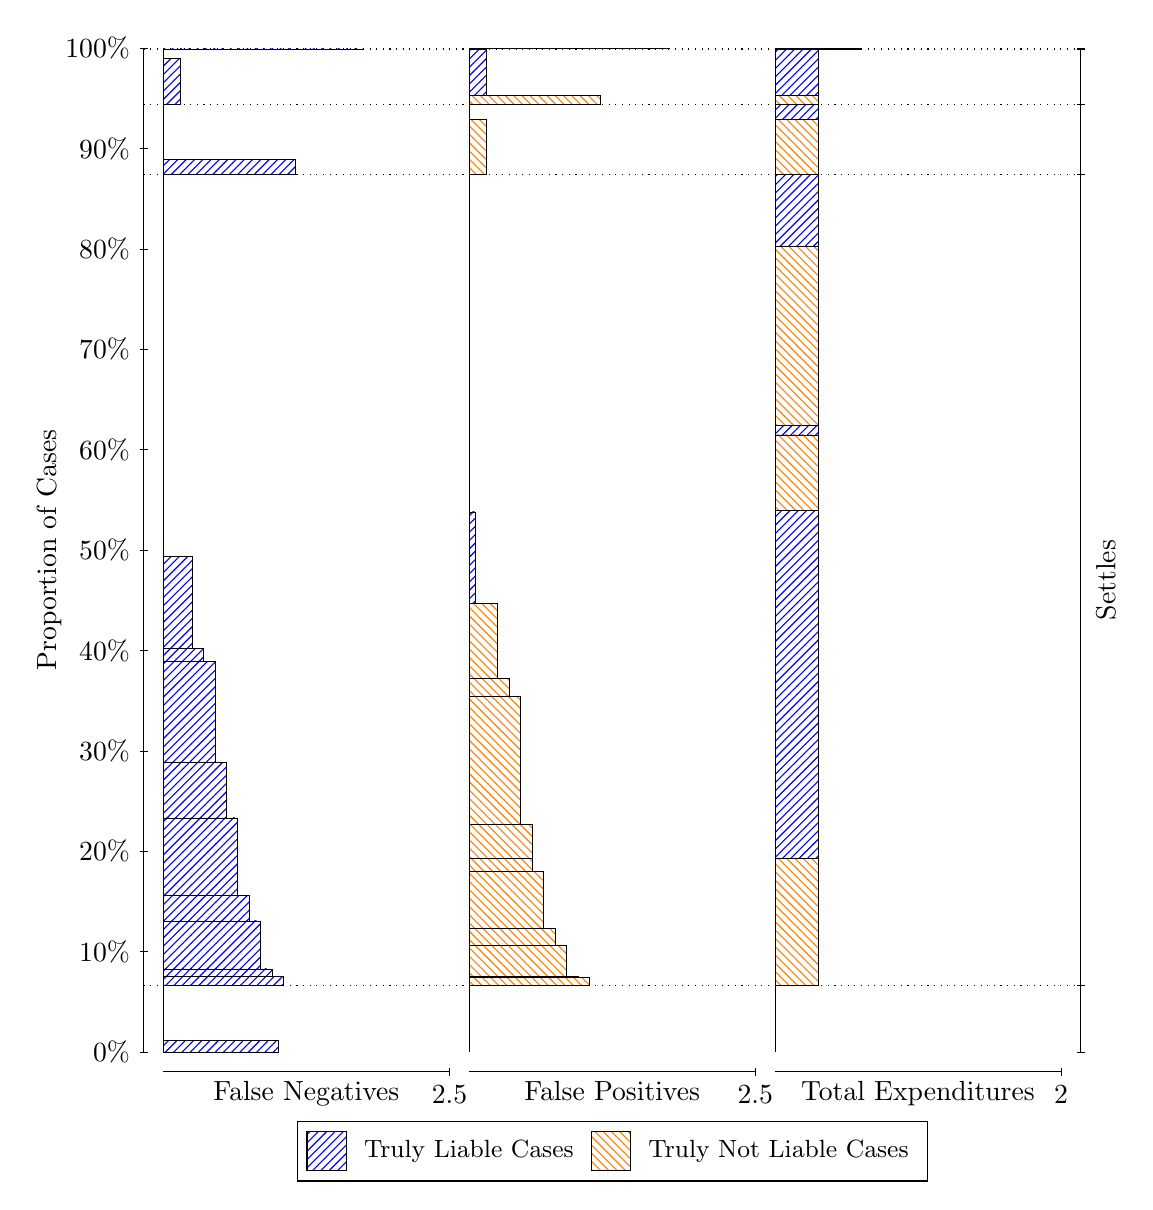
\begin{tikzpicture}
\draw[black, very thin] (1.5,1.75) -- (1.5,14.5);
\node[rotate=90, text=black, anchor=center] at (0.3, 8.125) {Proportion of Cases};
\draw[black, very thin] (1.45,1.75) -- (1.55,1.75);
\node[text=black, anchor=east] at (1.45, 1.75) {0\%};
\draw[black, very thin] (1.45,3.025) -- (1.55,3.025);
\node[text=black, anchor=east] at (1.45, 3.025) {10\%};
\draw[black, very thin] (1.45,4.3) -- (1.55,4.3);
\node[text=black, anchor=east] at (1.45, 4.3) {20\%};
\draw[black, very thin] (1.45,5.575) -- (1.55,5.575);
\node[text=black, anchor=east] at (1.45, 5.575) {30\%};
\draw[black, very thin] (1.45,6.85) -- (1.55,6.85);
\node[text=black, anchor=east] at (1.45, 6.85) {40\%};
\draw[black, very thin] (1.45,8.125) -- (1.55,8.125);
\node[text=black, anchor=east] at (1.45, 8.125) {50\%};
\draw[black, very thin] (1.45,9.4) -- (1.55,9.4);
\node[text=black, anchor=east] at (1.45, 9.4) {60\%};
\draw[black, very thin] (1.45,10.675) -- (1.55,10.675);
\node[text=black, anchor=east] at (1.45, 10.675) {70\%};
\draw[black, very thin] (1.45,11.95) -- (1.55,11.95);
\node[text=black, anchor=east] at (1.45, 11.95) {80\%};
\draw[black, very thin] (1.45,13.225) -- (1.55,13.225);
\node[text=black, anchor=east] at (1.45, 13.225) {90\%};
\draw[black, very thin] (1.45,14.5) -- (1.55,14.5);
\node[text=black, anchor=east] at (1.45, 14.5) {100\%};

\draw[black, very thin] (13.4,1.75) -- (13.4,14.5);
\draw[black, very thin] (13.35,1.75) -- (13.45,1.75);
\node[anchor=west] at (13.35, 1.75) {};
\draw[black, very thin] (13.35,2.5967) -- (13.45,2.5967);
\node[anchor=west] at (13.35, 2.5967) {};
\draw[black, very thin] (13.35,12.891) -- (13.45,12.891);
\node[anchor=west] at (13.35, 12.891) {};
\draw[black, very thin] (13.35,13.782) -- (13.45,13.782);
\node[anchor=west] at (13.35, 13.782) {};
\draw[black, very thin] (13.35,14.486) -- (13.45,14.486);
\node[anchor=west] at (13.35, 14.486) {};
\draw[black, very thin] (13.35,14.493) -- (13.45,14.493);
\node[anchor=west] at (13.35, 14.493) {};
\draw[black, very thin] (13.35,14.5) -- (13.45,14.5);
\node[anchor=west] at (13.35, 14.5) {};

\draw[black, very thin, pattern color=blue, pattern=north east lines] (1.75,1.75) rectangle (3.2033,1.8957);
\draw[black, very thin, pattern color=orange, pattern=north west lines] (1.75,1.8957) rectangle (1.75,2.5967);
\draw[black, very thin, pattern color=blue, pattern=north east lines] (1.75,2.5967) rectangle (3.276,2.7136);
\draw[black, very thin, pattern color=blue, pattern=north east lines] (1.75,2.7136) rectangle (3.1307,2.805);
\draw[black, very thin, pattern color=blue, pattern=north east lines] (1.75,2.805) rectangle (2.9853,3.4139);
\draw[black, very thin, pattern color=blue, pattern=north east lines] (1.75,3.4139) rectangle (2.84,3.7374);
\draw[black, very thin, pattern color=blue, pattern=north east lines] (1.75,3.7374) rectangle (2.6947,4.7216);
\draw[black, very thin, pattern color=blue, pattern=north east lines] (1.75,4.7216) rectangle (2.5493,5.4299);
\draw[black, very thin, pattern color=blue, pattern=north east lines] (1.75,5.4299) rectangle (2.404,6.7092);
\draw[black, very thin, pattern color=blue, pattern=north east lines] (1.75,6.7092) rectangle (2.2587,6.8795);
\draw[black, very thin, pattern color=blue, pattern=north east lines] (1.75,6.8795) rectangle (2.1133,8.0401);
\draw[black, very thin, pattern color=orange, pattern=north west lines] (1.75,8.0401) rectangle (1.75,12.891);
\draw[black, very thin, pattern color=blue, pattern=north east lines] (1.75,12.891) rectangle (3.4213,13.082);
\draw[black, very thin, pattern color=orange, pattern=north west lines] (1.75,13.082) rectangle (1.75,13.782);
\draw[black, very thin, pattern color=blue, pattern=north east lines] (1.75,13.782) rectangle (1.968,14.37);
\draw[black, very thin, pattern color=orange, pattern=north west lines] (1.75,14.37) rectangle (1.75,14.486);
\draw[black, very thin, pattern color=blue, pattern=north east lines] (1.75,14.486) rectangle (4.2933,14.489);
\draw[black, very thin, pattern color=orange, pattern=north west lines] (1.75,14.489) rectangle (1.75,14.493);
\draw[black, very thin, pattern color=orange, pattern=north west lines] (1.75,14.493) rectangle (1.75,14.496);
\draw[black, very thin, pattern color=blue, pattern=north east lines] (1.75,14.496) rectangle (1.75,14.5);
\draw[black, very thin, pattern color=orange, pattern=north west lines] (5.6333,1.75) rectangle (5.6333,2.451);
\draw[black, very thin, pattern color=blue, pattern=north east lines] (5.6333,2.451) rectangle (5.6333,2.5967);
\draw[black, very thin, pattern color=orange, pattern=north west lines] (5.6333,2.5967) rectangle (7.1593,2.6942);
\draw[black, very thin, pattern color=orange, pattern=north west lines] (5.6333,2.6942) rectangle (7.014,2.7148);
\draw[black, very thin, pattern color=orange, pattern=north west lines] (5.6333,2.7148) rectangle (6.8687,3.1012);
\draw[black, very thin, pattern color=orange, pattern=north west lines] (5.6333,3.1012) rectangle (6.7233,3.3172);
\draw[black, very thin, pattern color=orange, pattern=north west lines] (5.6333,3.3172) rectangle (6.578,4.0458);
\draw[black, very thin, pattern color=orange, pattern=north west lines] (5.6333,4.0458) rectangle (6.4327,4.2087);
\draw[black, very thin, pattern color=orange, pattern=north west lines] (5.6333,4.2087) rectangle (6.4327,4.6436);
\draw[black, very thin, pattern color=orange, pattern=north west lines] (5.6333,4.6436) rectangle (6.2873,6.2613);
\draw[black, very thin, pattern color=orange, pattern=north west lines] (5.6333,6.2613) rectangle (6.142,6.4901);
\draw[black, very thin, pattern color=orange, pattern=north west lines] (5.6333,6.4901) rectangle (5.9967,7.4477);
\draw[black, very thin, pattern color=blue, pattern=north east lines] (5.6333,7.4477) rectangle (5.706,8.6083);
\draw[black, very thin, pattern color=blue, pattern=north east lines] (5.6333,8.6083) rectangle (5.6333,12.891);
\draw[black, very thin, pattern color=orange, pattern=north west lines] (5.6333,12.891) rectangle (5.8513,13.591);
\draw[black, very thin, pattern color=blue, pattern=north east lines] (5.6333,13.591) rectangle (5.6333,13.782);
\draw[black, very thin, pattern color=orange, pattern=north west lines] (5.6333,13.782) rectangle (7.3047,13.899);
\draw[black, very thin, pattern color=blue, pattern=north east lines] (5.6333,13.899) rectangle (5.8513,14.486);
\draw[black, very thin, pattern color=orange, pattern=north west lines] (5.6333,14.486) rectangle (5.6333,14.491);
\draw[black, very thin, pattern color=blue, pattern=north east lines] (5.6333,14.491) rectangle (5.6333,14.493);
\draw[black, very thin, pattern color=orange, pattern=north west lines] (5.6333,14.493) rectangle (8.1767,14.496);
\draw[black, very thin, pattern color=blue, pattern=north east lines] (5.6333,14.496) rectangle (6.7233,14.5);
\draw[black, very thin, pattern color=orange, pattern=north west lines] (9.5167,1.75) rectangle (9.5167,2.451);
\draw[black, very thin, pattern color=blue, pattern=north east lines] (9.5167,2.451) rectangle (9.5167,2.5967);
\draw[black, very thin, pattern color=orange, pattern=north west lines] (9.5167,2.5967) rectangle (10.062,4.2087);
\draw[black, very thin, pattern color=blue, pattern=north east lines] (9.5167,4.2087) rectangle (10.062,8.6283);
\draw[black, very thin, pattern color=orange, pattern=north west lines] (9.5167,8.6283) rectangle (10.062,9.5859);
\draw[black, very thin, pattern color=blue, pattern=north east lines] (9.5167,9.5859) rectangle (10.062,9.7028);
\draw[black, very thin, pattern color=orange, pattern=north west lines] (9.5167,9.7028) rectangle (10.062,11.984);
\draw[black, very thin, pattern color=blue, pattern=north east lines] (9.5167,11.984) rectangle (10.062,12.891);
\draw[black, very thin, pattern color=orange, pattern=north west lines] (9.5167,12.891) rectangle (10.062,13.591);
\draw[black, very thin, pattern color=blue, pattern=north east lines] (9.5167,13.591) rectangle (10.062,13.782);
\draw[black, very thin, pattern color=orange, pattern=north west lines] (9.5167,13.782) rectangle (10.062,13.899);
\draw[black, very thin, pattern color=blue, pattern=north east lines] (9.5167,13.899) rectangle (10.062,14.486);
\draw[black, very thin, pattern color=orange, pattern=north west lines] (9.5167,14.486) rectangle (10.607,14.491);
\draw[black, very thin, pattern color=blue, pattern=north east lines] (9.5167,14.491) rectangle (10.607,14.493);
\draw[black, very thin, pattern color=orange, pattern=north west lines] (9.5167,14.493) rectangle (10.607,14.496);
\draw[black, very thin, pattern color=blue, pattern=north east lines] (9.5167,14.496) rectangle (10.607,14.5);
\draw[black, dotted] (1.5,2.5967) -- (13.4,2.5967);
\draw[black, dotted] (1.5,12.891) -- (13.4,12.891);
\draw[black, dotted] (1.5,13.782) -- (13.4,13.782);
\draw[black, dotted] (1.5,14.486) -- (13.4,14.486);
\draw[black, dotted] (1.5,14.493) -- (13.4,14.493);
\draw[black, very thin] (1.75,1.5) -- (5.3833,1.5);
\node[text=black, anchor=north] at (3.5667, 1.5) {False Negatives};
\draw[black, very thin] (5.3833,1.45) -- (5.3833,1.55);
\node[text=black, anchor=north] at (5.3833, 1.45) {2.5};

\draw[black, very thin] (5.6333,1.5) -- (9.2667,1.5);
\node[text=black, anchor=north] at (7.45, 1.5) {False Positives};
\draw[black, very thin] (9.2667,1.45) -- (9.2667,1.55);
\node[text=black, anchor=north] at (9.2667, 1.45) {2.5};

\draw[black, very thin] (9.5167,1.5) -- (13.15,1.5);
\node[text=black, anchor=north] at (11.333, 1.5) {Total Expenditures};
\draw[black, very thin] (13.15,1.45) -- (13.15,1.55);
\node[text=black, anchor=north] at (13.15, 1.45) {2};


\node[text=black, centered, rotate=90] at (13.72, 7.7439) {Settles};





\draw (7.449999999999999,1.5) node[draw=none] (baseCoordinate) {};
\begin{scope}[align=center]
        \matrix[scale=0.5, draw=black, below=0.5cm of baseCoordinate, nodes={draw}, column sep=0.1cm]{
            \node[rectangle, draw, minimum width=0.5cm, minimum height=0.5cm, pattern color=blue, pattern=north east lines] {}; &
            \node[draw=none, font=\small, text=black] (B) {Truly Liable Cases}; &
            \node[rectangle, draw, minimum width=0.5cm, minimum height=0.5cm, pattern color=orange, pattern=north west lines] {}; &
            \node[draw=none, font=\small, text=black] (B) {Truly Not Liable Cases}; \\
            };
\end{scope}

\end{tikzpicture}
\end{document}